\cia\vspace{-2 cm}
\section{\v Cerenkov efficiency}
\label{sec:cc_eff}
The GSIM simulation does not reproduce accurately the \v Cerenkov detector due to the
incomplete implementation of the detector optics. Furthermore the electron-pions contamination
is not present in the simulation.
For these reasons the pions and the PMT noise resulting in the peak at $1.0\; nphe$ illustrated in \F{fig:cccut}
do not show in the MonteCarlo, so that the real electrons lost with the cut $nphe < 2.5$ would not be recovered
with the acceptance calculation.

Studies \cite{bib:ludy}, \cite{bib:fid_e} of the $nphe$ spectra for the \v Cerenkov allow one
to determine a correction to the simulation that resolves this problem.
In \F{fig:ludy} the $nphe$ spectra is plotted for a particular electron $\phi$, $\theta$, $p$ and sector.
The distribution is fitted with the Poisson distribution 
\begin{equation}
y = A \Dfrac{L^{x/P}}{x/P}\,e^{L}
\end{equation}
with $A$, $P$, $L$ as parameters. The integral of the obtained function between $nphe =0$ and $nphe=25$ (shaded region) 
is a good estimate of the number of the electrons lost with the CC cut. The
the efficiency

\begin{equation}
E=1-\Dfrac{\int_0^{25} y \, {\rm d}x}{\int_{0}^{\infty} y \, {\rm d}x}
\end{equation}
is calculated. 
It was found that there are low efficiency regions around the fiducial cut, as one can expect,
but also at $\phi=0$, as is shown in \F{fig:fidu_ephis}.



An efficiency table is obtained with the following binning:
\vspace{0.4 cm}

\begin{table}[h]
\begin{center}
  \begin{tabular}{l l l}
$\bullet$ & $0<p<5$ GeV         & in steps of $0.5$ GeV. \\
$\bullet$ & $ 5^0<\theta<50^0$  & in steps of $5^0$. \\
$\bullet$ & $-25^0<\phi<25^0$ & in steps of $3.3^0$. \\

  \end{tabular}
 \end{center}
\end{table}


\begin{figure}[h]
  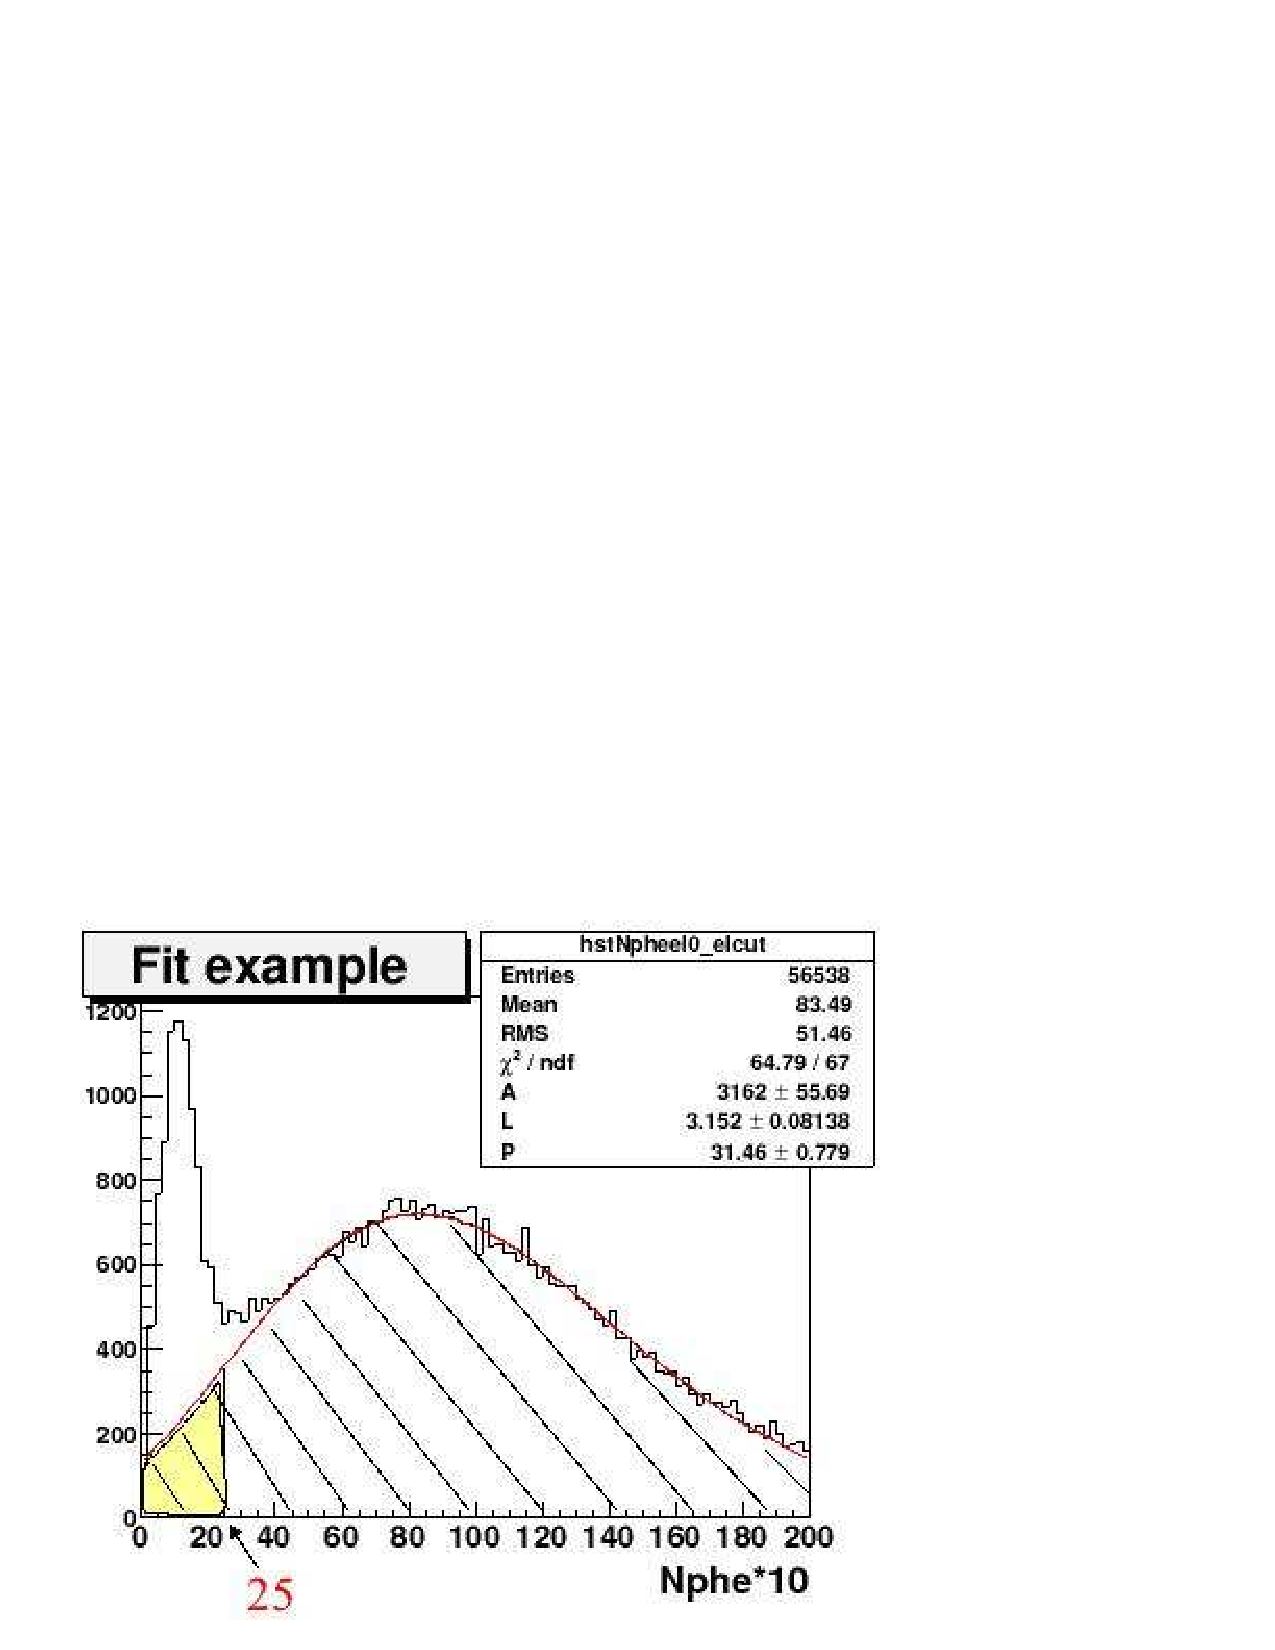
\includegraphics[width = 12cm, bb=-60 10 380 540]{data_reduction/img/ludy_cc_pic1}
  \caption[The $nphe$ spectra for $1.1 < p < 1.5$ GeV, $35^0 < \theta < 45^0$, $15^0 < \phi < 25^0$]
          { The $nphe*10$ spectra for $1.1 < p < 1.5$ GeV, $35^0 < \theta < 45^0$, $15^0 < \phi < 25^0$
	             and sector 1. The histogram is fitted for $nphe > 2.5$ with a Poisson distribution.
		     The integral of the obtained function between $nphe =0$ and $nphe=2.5$ (shaded region) 
		     is a good estimate of the number of the electron lost with the CC cut.
		     }
 \label{fig:ludy}
\end{figure}


When calculating the acceptance, each MonteCarlo event is weighted by the CC efficiency.

